\documentclass[12pt,a4paper]{article}
\usepackage[centertags]{amsmath}
\usepackage{graphicx}
\usepackage{caption3}
\usepackage{misccorr}
\usepackage{epsfig}
\usepackage{indentfirst}
\usepackage{ulem}
\usepackage[utf8]{inputenc}
\usepackage[english, russian]{babel}
\usepackage{setspace}
\usepackage{amssymb,amsfonts,amsmath,mathtext,braket,stmaryrd,mathrsfs}
\usepackage{cite}
\usepackage{subfigure}
\bibliographystyle{iopart-num}
\usepackage{geometry} % пакет для задания полей страницы командой \geometry
\geometry{left=3cm,right=1.5cm,top=2cm,bottom=2cm}
\numberwithin{equation}{section}
\DeclareMathOperator{\sign}{sign}
\DeclareMathOperator{\rot}{rot}
\DeclareMathOperator{\diver}{div}
\DeclareMathOperator{\w}{w}
\DeclareMathOperator{\Q}{Q}
\DeclareMathOperator{\Z}{Z}
\DeclareMathOperator{\F}{F}
\DeclareMathOperator{\M}{M}
\DeclareMathOperator{\q}{q}
\DeclareMathOperator{\g}{g}
\DeclareMathOperator{\h}{h}
\DeclareMathOperator{\e}{e}
\DeclareMathOperator{\vp}{\mathbf {v.p.}}
\makeatletter
\renewcommand \thesection {\@arabic\c@section}
\renewcommand\thesubsection {\thesection.\@arabic\c@subsection}
\renewcommand{\theequation}{\thesection.\arabic{equation}}
%\renewcommand{\thefigure}{\thesection.\arabic{figure}}
\linespread{1.3} % полтора интервала. Если 1.6, то два интервала
\renewcommand{\appendix}{\setcounter{section}{0}\gdef\thesection{\@Alph\c@section}}


\pagestyle{plain}

\begin{document}
\section{Постановка задачи}
Рассмотрим проникновение H-волны в неоднородную холодную плазму, образованную при многофотонной ионизации инертных газов. Одним из случаев неоднородной плазмы является плоскослоистая среда, в которой плотность изменяется только в одном направлении. Выберем систему координат таким образом, что падающая электромагнитная волна имеет вид $\bm{E}\left(z,t\right) =(1/2)\left(E_0,0,0\right)\cdot\exp\left[-i\omega\left(t-z/c\right)\right]+c.c.$, где. $c$ -- скорость света,  $\omega$ -- частота. Фотоионизованная плазма занимает полупространство $z>0$ и имеет распределение фотоэлектронов вида 
\begin{equation}
\label{fr}
    f_0(v, z) = \frac{n\left(z\right)}{4\pi v_0^2}\delta\left(v-v_0\right).
\end{equation}
При этом плотность плазмы $n\to 0$ при $z\to0$ и линейно возрастает до величины $n\left(L\right) = n_0$, после чего при $z>L$ остается постоянной. Электромагнитная волна порождает в плазме направленное вдоль оси $ox$ электрическое поле вида $(1/2)\bm{E}\left(z\right)\cdot\exp\left(-i\omega t\right)+c.c.$ и приводит к малому возмущению функции распределения фотоэлектронов по скоростям вида $(1/2)\,\delta f(\mathbf v,z)\exp\left(-i\omega t\right)+c.c$. Рассмотрим случай, когда частота падающей электромагнитной волны достаточно велика $$ \frac{v_0}{c}\ll \frac{\omega}{\omega_L}.$$ В этом случае дисперсионными поправками можно пренебречь. Поэтому для определения $\delta f\left(\mathbf v,z\right)$ воспользуемся следующим линеаризованным кинетическим уравнением с интегралом столкновений, описывающим релаксацию по направлениям скорости фотоэлектронов без изменения их энергии,
\begin{equation}
\label{kinetic}
    -i\omega\delta f(\mathbf v,z)+\frac{ev_x E\left(z\right)}{mv}\frac{\partial f_0(v, z)}{\partial v}= -\nu\left(v\right) \left[\delta f(\mathbf v,z)-\int \frac{d\Omega}{4\pi}\delta f(\mathbf v,z)\right],
\end{equation}
где $e$ — заряд электрона, $d\Omega$ -- элемент телесного угла.
Для определения поля в плазме воспользуемся самосогласованной системой уравнений Максвелла и уравнения \eqref{kinetic}. Тогда получим
\begin{equation}
    \label{field}
    \frac{d^2E}{dz^2}+\frac{\omega^2}{c^2}E = -\frac{4\pi i \omega}{c^2}j,
\end{equation}
где выражение для плотности тока в плазме с учетом зависимости частоты столкновений фотоэлектронов от их скорости имеет вид
\begin{equation}
    \label{current}
    j = \frac{e^2}{m} \int d\bm{v} \frac{v_x^2}{v}\frac{\partial f_0}{\partial v} \frac{E\left(z\right)}{i\omega-\nu\left(v\right)}.
\end{equation}
Вычислив интеграл в выражении для плотности тока \eqref{current}, уравнение \eqref{field} можно переписать в виде
\begin{equation}
    \label{field2}
    \frac{d^2E}{dz^2}+\frac{\omega^2}{c^2}\varepsilon\left(\omega, z\right)E = 0,
\end{equation}
где диэлектрическая проницаемость имеет вид
\begin{equation}
    \label{perm_fin}
    \varepsilon(\omega, z)=1-\frac{\omega_L^2\left(z\right)}{\omega\left(\omega+i\nu\right) }\left[1-i\frac{\alpha}{3}\frac{\nu}{\omega+i\nu}\right].
\end{equation}
Здесь $\omega_L\left(z\right) = \sqrt{4\pi n\left(z\right)e^2/m}$ — ленгмюровская частота электронов, $\nu\equiv\nu\left(v_0\right),\alpha=\partial \ln\nu/\partial \ln v_0%|_{v = v_0}%
$ — величина, определяющаяся средней энергией фотоэлектронов и видом зависимости транспортного сечения рассеяния от энергии. %Поскольку плотность электронов является линейной функцией координаты, то уравнение \eqref{field2} подстановкой 
%\begin{equation}
%    \label{xi}
%    \xi = \left(\frac{4\pi \beta e^2\omega}{mc^2\left(\omega+i\nu\right)\left(1-i\alpha/3 \left(\nu/\left(\omega+i\nu\right)\right)\right)^2}\right)^{1/3}\left[\frac{m\omega\left(\omega+i\nu\right)}{4\pi\beta e^2} -z\left(1-i\frac{\alpha}{3}\frac{\nu}{\omega+i\nu}\right)\right]
%\end{equation} может быть приведено к уравнению Эйри
%\begin{equation}
%    \label{Aery}
%    \frac{d^2 E}{d\xi^2}+\xi E = 0.
%\end{equation}
%В \eqref{xi} $\beta$ - коэффициент пропорциональности между плотностью электронов и координатой $z$.
%Решение уравнения \eqref{Aery}, убывающее на бесконечности имеет вид
%\begin{equation}
%    \label{solve}
%    E\left(\xi\right) = \frac{3A}{\pi}\int_{0}^{\infty} \cos\left(\frac{y^3}{3}-\xi y\right)dy,
%\end{equation}
%где коэффициент $A$ определяется из граничных условий.
\section{Общее решение для малых частот столкновений}
В разреженной плазме частоты столкновений фотоэлектронов сравнительно малы и интерес представляют условия, когда $\omega \gg \nu$. В этом случае
диэлектрическую проницаемость \eqref{perm_fin} можно переписать в виде
\begin{equation}
    \label{perm_nu}
    \varepsilon(\omega, z)=1-\frac{\omega_L^2\left(z\right)}{\omega^2}\left[1-i\left(1+\frac{\alpha}{3}\right)\frac{\nu}{\omega}\right].
\end{equation}

Область, занимаемую плазмой, можно разделить на две части, - ту, где плотность электронов меняется линейно и ту, где она является постоянной величиной. В области $0<z<L$ выражение \eqref{perm_nu} можно переписать в виде
\begin{equation}
    \varepsilon(\omega, z) = 1 - \frac{\omega_L^2}{\omega^2}\frac{z}{L}\left[1-i\left(1+\frac{\alpha}{3}\right)\frac{\nu}{\omega}\right].
\end{equation}
Поскольку диэлектрическая проницаемость является линейной функцией координаты, то уравнение \eqref{field2} подстановкой 
\begin{equation}
    \xi = \left(\frac{\omega^2}{z_0 c^2}\right)^{1/3}\left(z-z_0\right)
\end{equation}
может быть приведено к уравнению Эйри
\begin{equation}
    \label{Aery}
    \frac{d^2 E}{d\xi^2}-\xi E = 0,
\end{equation}
где 
\begin{equation}
    z_0 = \frac{\omega^2}{\omega_L^2}L\left[1+i\left(1+\alpha/3\right)\nu/\omega\right],
\end{equation}
а $\omega_L \equiv \omega_L\left(L\right)$. Решением уравнения \eqref{Aery} будет сумма двух функций Эйри  с коэффициентами, определяемыми из граничных условий,
\begin{equation}
    \label{field_L}
    E\left(\xi\right) = C_1 Ai\left(\xi\right)+C_2 Bi\left(\xi\right).
\end{equation}

В области $z>L$ плотность электронов постоянна, поэтому диэлектрическая проницаемость перестает зависеть от координаты $z$ и решением уравнения \eqref{field} будет убывающая экспоненциально волна вида
\begin{equation}
    \label{field_inf}
    E\left(z\right) = C_3\exp\left[-\frac{\sqrt{\omega_L^2-\omega^2}}{c}\left(1-\frac{i}{2}\left(1+\frac{\alpha}{3}\right)\frac{\omega_L^2}{\omega_L^2-\omega^2}\frac{\nu}{\omega}\right)z\right].
\end{equation}

Для того, чтобы найти неизвестные коэффициенты $C_1, C_2, C_3$ воспользуемся граничными условиями. На границе плазмы $z=0$ тангенциальные компоненты электрического и магнитного полей непрерывны 
\begin{equation}
\label{bound}
    E_0+E_r=E(+0), \qquad  E_0-E_r=B(+0),
\end{equation}
где $E_r$ - амплитуда волны, уходящей от границы плазмы в область $z<0$. Аналогично и при $z=L$ поле и его производные должны быть непрерывными. Таким образом, получаем систему из 4 уравнений на 4 неизвестных. Обозначим $\gamma = 1-i/2\left(1+\alpha/3\right)\omega_L^2\nu/\omega\left(\omega_L^2-\omega^2\right),$ $\xi\left(0\right) = \xi_0, \xi\left(L\right) = \xi_L$. Тогда
\begin{equation}
    \label{system}
    \begin{cases}
    E_0+E_r = C_1 Ai\left(\xi_0\right)+C_2 Bi\left(\xi_0\right), \\
    E_0-E_r=-i\frac{c}{\omega}\left[Ai\,'_z\left(\xi_0\right)+C_2 Bi\,'_z\left(\xi_0\right)\right],\\
    C_1 Ai\left(\xi_L\right)+C_2 Bi\left(\xi_L\right)=C_3\exp\left[-\frac{\sqrt{\omega_L^2-\omega^2}}{c}\gamma L\right], \\
    C_1 Ai\,'_z\left(\xi_L\right)+C_2 Bi\,'_z\left(\xi_L\right)=  C_3\left(-\frac{\sqrt{\omega_L^2-\omega^2}}{c}\gamma \right)\exp\left[-\frac{\sqrt{\omega_L^2-\omega^2}}{c}\gamma L\right].
    
    \end{cases}
\end{equation}

Учитывая зависимость $\xi$ от $z$ при взятии производных от функций Эйри
\begin{equation}
    \label{}
    Ai\,'_z\left(\xi\left(z\right)\right) = \left(\frac{\omega^2}{z_0 c^2}\right)^{1/3}Ai\,'\left(\xi\right) \equiv \xi' Ai\,'\left(\xi\right),
\end{equation}
Найдем связь между коэффициентами $C_1$ и $C_2$ путем исключения $C_3$. Тогда
\begin{equation}
      \label{C1C2}
      \begin{array}{lcl}
    C_1\left[Ai\left(\xi_L\right)\frac{\sqrt{\omega_L^2-\omega^2}}{c}\gamma+\xi'Ai\,'\left(\xi_L\right)\right] = \\ -C_2\left[Bi\left(\xi_L\right)\frac{\sqrt{\omega_L^2-\omega^2}}{c}\gamma+\xi'Bi\,'\left(\xi_L\right)\right]
\end{array}
\end{equation}
Исключая $E_r$ из первых двух уравнений системы \eqref{system} и подставляя связь \eqref{C1C2}, получим для коэффициентов $C_1$ и $C_2$ следующие выражения
\begin{equation}
    \label{C1_common}
    \begin{array}{lcl}
         C_1 = -2E_0\left[Bi\left(\xi_L\right)\frac{\sqrt{\omega_L^2-\omega^2}}{c}\gamma+\xi'Bi\,'\left(\xi_L\right)\right]\times \\
       \left\{\left[Bi\left(\xi_0\right)-i\left(\frac{c}{\omega z_0}\right)^{1/3}Bi\,'\left(\xi_0\right)\right]\left[Ai\left(\xi_L\right)\frac{\sqrt{\omega_L^2-\omega^2}}{c}\gamma+\xi'Ai\,'\left(\xi_L\right)\right] - \right.\\ 
       \left.\left[Ai\left(\xi_0\right)-i\left(\frac{c}{\omega z_0}\right)^{1/3}Ai\,'\left(\xi_0\right)\right]\left[Bi\left(\xi_L\right)\frac{\sqrt{\omega_L^2-\omega^2}}{c}\gamma+\xi'Bi\,'\left(\xi_L\right)\right]\right\}^{-1},
    \end{array}
\end{equation}

\begin{equation}
    \label{C2_common}
    \begin{array}{lcl}
         C_2 = 2E_0\left[Ai\left(\xi_L\right)\frac{\sqrt{\omega_L^2-\omega^2}}{c}\gamma+\xi'Ai\,'\left(\xi_L\right)\right]\times \\
       \left\{\left[Bi\left(\xi_0\right)-i\left(\frac{c}{\omega z_0}\right)^{1/3}Bi\,'\left(\xi_0\right)\right]\left[Ai\left(\xi_L\right)\frac{\sqrt{\omega_L^2-\omega^2}}{c}\gamma+\xi'Ai\,'\left(\xi_L\right)\right] - \right.\\ 
       \left.\left[Ai\left(\xi_0\right)-i\left(\frac{c}{\omega z_0}\right)^{1/3}Ai\,'\left(\xi_0\right)\right]\left[Bi\left(\xi_L\right)\frac{\sqrt{\omega_L^2-\omega^2}}{c}\gamma+\xi'Bi\,'\left(\xi_L\right)\right]\right\}^{-1}.
    \end{array}
\end{equation}

Определим коэффициент отражения на границе плазмы как
\begin{equation}
    \label{refl}
    R = \frac{E_r}{E_0}.
\end{equation}
Вычислив $E_r$ из системы \eqref{system} и подставляя значения коэффициентов $C_1$ и $C_2$, получим в общем виде выражение для коэффициента отражения
\begin{equation}
\label{coeff}
\begin{array}{lcl}
  R = \left\{\left[Bi\left(\xi_0\right)+i\left(\frac{c}{\omega z_0}\right)^{1/3}Bi\,'\left(\xi_0\right)\right]\left[Ai\left(\xi_L\right)\frac{\sqrt{\omega_L^2-\omega^2}}{c}\gamma+\xi'Ai\,'\left(\xi_L\right)\right] - \right. \\
  \left.\left[Ai\left(\xi_0\right)+i\left(\frac{c}{\omega z_0}\right)^{1/3}Ai\,'\left(\xi_0\right)\right]\left[Bi\left(\xi_L\right)\frac{\sqrt{\omega_L^2-\omega^2}}{c}\gamma+\xi'Bi\,'\left(\xi_L\right)\right]\right\}\times \\
  \left\{\left[Bi\left(\xi_0\right)-i\left(\frac{c}{\omega z_0}\right)^{1/3}Bi\,'\left(\xi_0\right)\right]\left[Ai\left(\xi_L\right)\frac{\sqrt{\omega_L^2-\omega^2}}{c}\gamma+\xi'Ai\,'\left(\xi_L\right)\right] \right. -\\
   \left.\left[Ai\left(\xi_0\right)-i\left(\frac{c}{\omega z_0}\right)^{1/3}Ai\,'\left(\xi_0\right)\right]\left[Bi\left(\xi_L\right)\frac{\sqrt{\omega_L^2-\omega^2}}{c}\gamma+\xi'Bi\,'\left(\xi_L\right)\right]\right\}^{-1}.
\end{array}
\end{equation}

Коэффициент поглощения $A\left(\omega\right)$, характеризующий долю переданной плазме энергии падающей волны, имеет вид
\begin{equation}
    \label{absorp_common}
    A\left(\omega\right) = 1-\left|R\right|^2.
\end{equation}

\section{Асимптотические выражения для коэффициента поглощения}
Свойства функций Эйри позволяют написать асимптотические выражения для электрического поля внутри плазмы. В общие выражения для $E\left(z\right)$ и коэффициента поглощения входят значения функций Эйри в точках $\xi_0$ и $\xi_L$, абсолютные значения которых имеют вид
\begin{equation}
\label{xi}
    |\xi_0|\approx \frac{\omega^2}{\omega_L^2}\left(\frac{\omega_L}{c}L\right)^{2/3},\quad |\xi_L|\approx \left(\frac{\omega_L}{c}L\right)^{2/3}.
\end{equation}
Из \eqref{xi} видно, что в случае, когда частота падающего электромагнитного излучения меньше плазменной, $|\xi_0|<|\xi_L|$. Исходя из соотношения между значениями \eqref{xi} и единицей, можно рассмотреть три предельных случая в зависимости от ширины слоя переменной плотности.
\subsection{Случай узкого слоя переменной плотности}
 Рассмотрим случай, когда ширина слоя меньше электромагнитного масштаба
\begin{equation}
    \label{cond1}
    L<\frac{c}{\omega_L}.
\end{equation}
При таком условии $|\xi_L|\ll 1$, а следовательно и $|\xi_0|\ll 1$. Для малых аргументов функций Эйри справедливо следующее асимптотическое разложение [ссылка на Абрамовица]
\begin{equation}
    \label{asymp_small}
    Ai\left(\xi\right) = \frac{1}{3^{2/3}\Gamma\left(2/3\right)}-\frac{1}{3^{1/3}\Gamma\left(1/3\right)}\xi, \quad 
    Bi\left(\xi\right) = \sqrt{3}\left(\frac{1}{3^{2/3}\Gamma\left(2/3\right)}+\frac{1}{3^{1/3}\Gamma\left(1/3\right)}\xi\right).
\end{equation}
Тогда, учитывая значения функций Эйри  \eqref{asymp_small}, имеем выражение для поля внутри слоя переменной плотности 
\begin{equation}
    \label{E1_small}
     E\left(z\right)= 2E_0\frac{\left(L-z\right)\sqrt{\omega_L^2-\omega^2} \gamma/c+1}{\left(L+i\frac{c}{\omega}\right)\frac{\sqrt{\omega_L^2-\omega^2}}{c}\gamma+1}.
\end{equation}
А в области $z>L$ поле имеет вид
\begin{equation}
    \label{E2_small}
     E\left(z\right) = 2E_0   \frac{\exp\left[-\frac{\sqrt{\omega_L^2-\omega^2}}{c}\gamma\left(z-L\right)\right]}{\left(L+i\frac{c}{\omega}\right)\frac{\sqrt{\omega_L^2-\omega^2}}{c}\gamma+1}.
\end{equation}
Таким образом, поле внутри слоя переменной плотности убывает линейно внутрь плазмы, а, когда плотность плазмы становится постоянной, убывает экспоненциальным образом. Точное решение для абсолютного значения поля внутри плазмы $E\left(z\right)$ продемонстрировано на рис.\ref{E_small}. График на рисунке \ref{E_small} построен с использованием общих выражений \eqref{C1_common} и \eqref{C2_common} для параметров $\alpha = 4.8$, что соответствует плазме, полученной при трехфотонной ионизации ксенона со средней энергией фотоэлектронов $\epsilon_0=2.87\text{eV}$ [ссылка на Попова], частоты падающего поля $\omega = 0.5\omega_L$, частоты столкновений фотоэлектронов $\nu = 0.01 \omega_L$ и ширины слоя $L = 1/3 c/\omega_L$. Точками на оси $x$ обозначены характерные масштабы рассматриваемой задачи, и введено обозначени $\delta = c/\omega_L$. Как видно из рисунка \eqref{E_small} поле внутрь плазмы проникает на расстояние порядка нескольких электромагнитных масштабов.
\begin{figure}[!ht]	
	\center{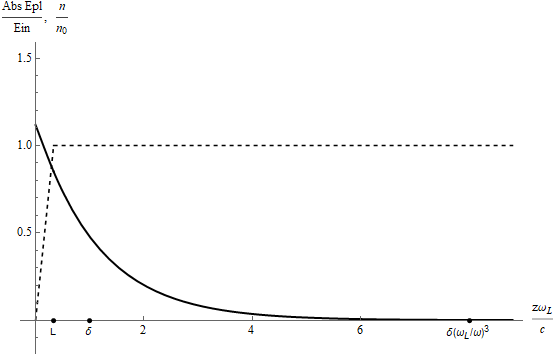
\includegraphics[scale=0.65]{thin_layer.png}}
	\caption{Зависимость абсолютного значения  поля внутри плазмы от расстояния до границы плазмы $z=0$.}
    \label{E_small}
\end{figure}
Из выражения \eqref{coeff} получим коэффициент отражения в виде

\begin{equation}
    \label{coeff1_small}
    R = -\frac{i\sqrt{\omega_L^2-\omega^2}\gamma/\omega - 1}{i\sqrt{\omega_L^2-\omega^2}\gamma/\omega + 1}.
\end{equation}
Тогда, учитывая связь коэффициента отражения с коэффициентом поглощения и подставляя выражение для $\gamma$, имеем
\begin{equation}
\label{coeff2_small}
    A\left(\omega\right) = 2 \frac{\nu}{\sqrt{\omega_L^2-\omega^2}}\left(1+\frac{\alpha}{3}\right).
\end{equation}
Этот же результат получается, если рассматривать плазму с резкой границей, то есть $L \to 0$ [ссылка на нашу работу]. Таким образом, если в плазме, образованной при многофотонной ионизации инертного газа, размытие границы мало по сравнению с электромагнитным масштабом, то границу можно считать резкой.
\subsection{Случай промежуточной ширины слоя}
Поскольку $|\xi_0|<|\xi_L|$, то можно рассмотреть случай, когда $|\xi_0|\ll 1$, а $|\xi_L| \gg 1$. Такие параметры соответсвуют ширине слоя переменной плотности в пределах 
\begin{equation}
    \label{cond2}
    \frac{c}{\omega_L}<L<\frac{\omega_L^3}{\omega^3} \frac{c}{\omega_L}.
\end{equation}
Для больших аргументов функций Эйри имеют место следующие асимптотические выражения [Абрамовиц]
\begin{subequations}
\label{asymp_big}
\begin{align}
    Ai\left(\xi\right) &= \frac{1}{2\sqrt{\pi}\xi^{1/4}}\exp\left[-\frac{2}{3}\xi^{3/2}\right]\left(1-\frac{5}{48}\frac{1}{\xi^{3/2}}\right),& |\text{arg}\,\xi| <\pi, \label{asymp_big_a}
    \\ Bi\left(\xi\right) &= \frac{1}{\sqrt{\pi}\xi^{1/4}}\exp\left[\frac{2}{3}\xi^{3/2}\right]\left(1+\frac{5}{48}\frac{1}{\xi^{3/2}}\right),& |\text{arg}\, \xi| <\pi/3, \label{asymp_big_b}\\ 
    Ai\left(-\xi\right) &= \frac{1}{\sqrt{\pi}\xi^{1/4}}\sin\left(\frac{2}{3}\xi^{3/2}+\frac{\pi}{4}\right),& |\text{arg}\, \xi| <2\pi/3, \label{asymp_big_c} \\
    Bi\left(-\xi\right) &= \frac{1}{\sqrt{\pi}\xi^{1/4}}\cos\left(\frac{2}{3}\xi^{3/2}+\frac{\pi}{4}\right),& |\text{arg}\,\xi| <2\pi/3. \label{asymp_big_d}
\end{align}
\end{subequations}
В рассматриваемом случае $|\text{arg}\, \xi_L| <\pi/3$, поэтому для вычисления поля внутри плазмы для $Ai\left(\xi_L\right)$ и $Bi\left(\xi_L\right)$ воспользуемся формулами \eqref{asymp_big_a} и \eqref{asymp_big_b}, соответственно, а для $Ai\left(\xi_0\right), Bi\left(\xi_0\right)$ воспользуемся \eqref{asymp_small}. В данном случае коффициент $C_2$ много меньше, чем $C_1$, и слагаемое $C_2Bi\left(\xi\right)$ в выражении \eqref{field_L} является поправкой порядка $1/\xi_L$ к $C_1Ai\left(\xi\right)$ для всех значений $\xi$. Тогда поле внутри слоя переменной плотности можно представить в виде
\begin{eqnarray}
    E\left(z\right)\approx -2i E_0 3^{1/3} \Gamma\left(1/3\right)\left(\frac{\omega z_0}{c}\right)^{1/3}\left[ Ai\left(\xi\left(z\right)\right)+ \nonumber\right. \\
    +\left.\frac{7}{192}\left(\frac{\omega^2}{\omega_L^2-\omega^2}\right)^{3/2}\frac{c}{\omega z_0 \gamma^3}\exp\left[-\frac{4}{3}\frac{\omega z_0}{c}\left(\gamma^2\frac{\omega_L^2-\omega^2}{\omega^2}\right)^{3/2}\right]Bi\left(\xi\left(z\right)\right)\right]. 
    \label{E1_med}
\end{eqnarray}
Внутри плазмы с постоянной плотностью фотоэлектронов
\begin{eqnarray}
    \label{E2_med}
    E\left(z\right) \approx -iE_0 \frac{3^{1/3} \Gamma\left(1/3\right)}{\sqrt{\pi}}\left(\frac{\omega z_0}{c}\right)^{1/6}\left(\frac{z_0}{L}\right)^{1/4} \left(1+\frac{7}{192}\left(\frac{\omega^2}{\omega_L^2-\omega^2}\right)^{3/2}\frac{c}{\omega z_0 \gamma^3}\right) \times \nonumber\\
    \exp\left[-\frac{\sqrt{\omega_L^2-\omega^2}}{c}\gamma\left(z-L\right)-\frac{2}{3} \frac{\omega z_0}{c}\left(\gamma^2\frac{\omega_L^2-\omega^2}{\omega^2}\right)^{3/2}\right].
     \label{E2_med}
\end{eqnarray}
Таким образом, поле внутри слоя переменной плотности сначала линейно убывает внутрь плазмы до точки $z\omega_L/c \sim \left(L\omega_L/c\right)^{1/3$, а после начинает убывать экспоненицально. Точное решение для абсолютного значения поля внутри плазмы $E\left(z\right)$ продемонстрировано на рис.\ref{E_mid}. График на рисунке \ref{E_mid} построен с использованием общих выражений \eqref{C1_common} и \eqref{C2_common} для параметров $\alpha = 4.8$, частоты падающего поля $\omega = 0.5\omega_L$, частоты столкновений фотоэлектронов $\nu = 0.01 \omega_L$ и ширины слоя $L = 3 c/\omega_L$. Как видно из рисунка \eqref{E_mid}, поле проникает внутрь плазмы на расстояния много больше, чем в случае узкого слоя (см. рис. \ref{E_small}).
\begin{figure}[!ht]	
	\center{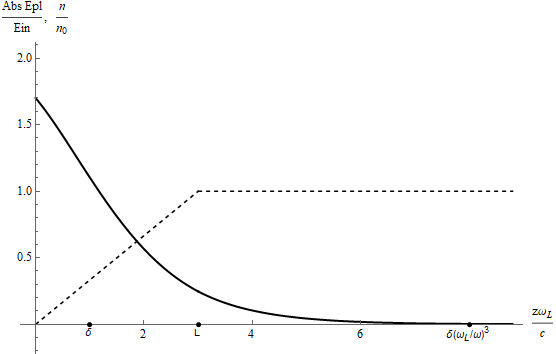
\includegraphics[scale=0.65]{mid_layer.png}}
	\caption{Зависимость абсолютного значения  поля внутри плазмы от расстояния до границы плазмы $z=0$.}
    \label{E_mid}
\end{figure}

Из выражения \eqref{coeff} получим коэффициент отражения в виде
\begin{equation}
    \label{coeff1_mid}
    R \approx \frac{\Gamma\left(1/3\right) - i\left(3c/\omega z_0\right)^{1/3}\Gamma\left(2/3\right)}{\Gamma\left(1/3\right) + i\left(3c/\omega z_0\right)^{1/3}\Gamma\left(2/3\right)}.
\end{equation}
Откуда следует, что коэффициент поглощения имеет вид 
\begin{equation}
    \label{coeff2_mid}
    A\left(\omega\right) \approx 4 \frac{\Gamma\left(1/3\right)}{3^{1/3}\Gamma\left(2/3\right)}\left(\frac{L\omega_L}{c}\right)^{1/3}\frac{\nu}{\omega_L}\left(1+\frac{\alpha}{3}\right).
\end{equation}
Сравнивая выражения \eqref{coeff2_small} и \eqref{coeff2_mid}, получаем, что в случае более широкого слоя переменной плотности коэффициент прохождения увеличивается в $\left(L\omega_L/c\right)^{1/3}$ раз в области частот падающего излучения, не близких к плазменной.
\subsection{Широкий слой}
Последний рассматриваемый случай имеет место, когда ширина слоя переменной плотности достаточно большая, а именно
\begin{equation}
    \label{cond3}
    \frac{\omega_L^3}{\omega^3}\frac{c}{\omega_L}<L.
\end{equation}

В этом случае абсолютные значения переменной $\xi$ на границах слоя $|\xi_0|, \, |\xi_L| \gg 1$. Учитывая значения $\arg \xi$, для границы $z=0$ воспользуемся выражениями \eqref{asymp_big_c} и \eqref{asymp_big_d}, а для $z=L$, как в предыдущем рассматриваемом случае, -- выражениями \eqref{asymp_big_a} и \eqref{asymp_big_b}. В данном случае, $\xi_L$ еще больше, чем в предыдущем разделе, поэтому можно положить коэффициент $C_2\approx 0$. Тогда поле внутри слоя имеет вид
\begin{equation}
  \label{E1_big}
  E\left(z\right) = 2E_0\sqrt{\pi}\left(\frac{\omega z_0}{c}\right)^{1/6}\exp\left[i\left(\frac{2}{3} \frac{\omega z_0}{c}-\frac{\pi}{4}\right)\right]Ai\left(\xi\left(z\right)\right).
\end{equation}
В области $z>L$, вычисляя коэффициент $C_3$ с учетом \eqref{E1_big}, получим
\begin{eqnarray}
    E\left(z\right) = E_0\left(\frac{1}{\gamma^2}\frac{\omega^2}{\omega_L^2-\omega^2}\right)^{1/4}\exp\left[-\frac{\sqrt{\omega_L^2-\omega^2}}{c}\gamma\left(z-L\right)+i\left(\frac{2}{3} \frac{\omega z_0}{c}-\frac{\pi}{4}\right)\right. \nonumber \\
    -\left.\frac{2}{3} \frac{\omega z_0}{c}\left(\gamma^2\frac{\omega_L^2-\omega^2}{\omega^2}\right)^{3/2}\right].
    \label{E2_big}
\end{eqnarray}
Учитывая \eqref{E1_big} и \eqref{E2_big}, поведение поля внутри плазмы сначала описывается периодической функцией, затем вблизи точки $L\omega^2/\omega_L^2$ убывающей линейно функцией и наконец затем экспоненциально убывающей функцией. Точное решение для абсолютного значения поля внутри плазмы $E\left(z\right)$ продемонстрировано на рис.\ref{E_big}. График на рисунке \ref{E_big} построен с использованием общих выражений \eqref{C1_common} и \eqref{C2_common} для параметров $\alpha = 4.8$, частоты падающего поля $\omega = 0.5\omega_L$, частоты столкновений фотоэлектронов $\nu = 0.01 \omega_L$ и ширины слоя $L = 15 c/\omega_L$. В этом случае, поле проникает еще глубже, чем в предущих рассматриваемых случаях. Однако затухание происходит еще до начала участка с постоянной плотностью фотоэлектронов.  
\begin{figure}[!ht]	
	\center{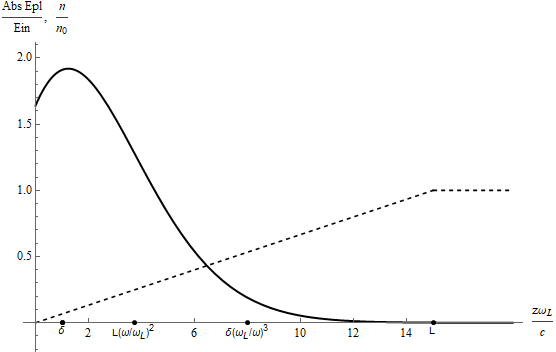
\includegraphics[scale=0.65]{thick_layer.png}}
	\caption{Зависимость абсолютного значения  поля внутри плазмы от расстояния до границы плазмы $z=0$.}
    \label{E_big}
\end{figure}

Коэффициент отражения в данном случае имеет вид 
\begin{equation}
    \label{coeff1_big}
    R = \exp\left[i\left(\frac{4}{3} \frac{\omega z_0}{c}-\frac{\pi}{2}\right)\right].
\end{equation}
Тогда для коэффициента поглощения имеем 
\begin{equation}
   \label{coeff2_big}
   A\left(\omega\right) = 1-\exp\left[-\frac{8}{3}\left(1+\alpha/3\right)\frac{\nu}{\omega_L}\frac{L\omega_L}{c}\frac{\omega^2}{\omega_L^2}\right].
\end{equation}
Таким образом, если $L\omega_L/c\cdot\omega^3/\omega_L^3\gg\omega/\nu$, то почти все поле поглощается плазмой, а в обратном случае поле почти целиком отражается.
\end{document}
